\documentclass{template/openetcs_article}
% Use the option "nocc" if the document is not licensed under Creative Commons
%\documentclass[nocc]{template/openetcs_article}
\usepackage{lipsum,url}
\usepackage{supertabular}
\usepackage{multirow}
\usepackage{color, colortbl}
\definecolor{gray}{rgb}{0.8,0.8,0.8}
\usepackage[modulo]{lineno}
\graphicspath{{./template/}{.}{./images/}}
\begin{document}
\frontmatter
\project{openETCS}

%Please do not change anything above this line
%============================



% The document metadata is defined below

%assign a report number here
\reportnum{OETCS/WP3/}

%define your workpackage here
\wp{Work-Package 3: ``Modeling''}

%set a title here
\title{OpenETCS SSRS Description of Work -DoW- }

%set a subtitle here
\subtitle{OpenETCS SSRS Task Force}

%set the date of the report here
\date{October 2012\\Revised March 2013}

%define a list of authors and their affiliation here
\author{Stanislas Pinte }
\affiliation{ERTMS Solutions}

\author{Baseliyous Jacob}

\affiliation{Deutsche Bahn AG / DB Netz AG\\
  openETCS Project Group \\
  Voelckerstrasse 5\\
  80939 Muenchen, Germany \\
  \\
  eMail: ProjectOffice@openETCS.org \\
  WebSite: www.openETCS.org}


% define the coverart
\coverart[width=350pt]{openETCS_EUPL}

%define the type of report
\reporttype{Description of work}


%\begin{abstract}
%define an abstract here
%  \lipsum[12-13]
%\end{abstract}

%=============================
\maketitle

%Modification history
%if you do not need a modification history table for your document simply comment out the eight lines below
%=============================
\section*{Modification History}
\tablefirsthead{
\hline 
\rowcolor{gray} 
Version & Section & Modification / Description & Author \\\hline}
\begin{supertabular}{| m{1.2cm} | m{1.2cm} | m{6.6cm} | m{4cm} |}
 & & & \\\hline
\end{supertabular}


\tableofcontents
\listoffiguresandtables
\newpage
%=============================

%Uncomment the next line if you need line numbers for tracebility when the document is in review
%\linenumbers
%=============================


% The actual document starts below this line
%=============================

%Start here









%Examples are below


\section{Abstract}
This taskforce will gather and sum up the necessary requirements, documents, variables and interfaces to develop a generic OBU kernel. In this case it is required to add a step of document between the SRS and the intended model of the OBU. 

The modeling of the SRS would require the following steps:
\begin{itemize}
  \item to define the scope of the model ( \textasciitilde the OBU kernel);
  \item	to provide an architecture for this model (functional and SW);
  \item to lift ambiguities;
  \item to detect errors and inconsistencies;
  \item to transform requirements into an executable content;
  \item to transform a natural language into a formal language.
\end{itemize}
Adding a step of documentation allows breaking these difficulties down. This step would be the Sub-System Requirement Specification. This step will allow the following:
\begin{itemize}
\item	to define the scope of the model (more or less the OBU kernel);
\item	to provide an architecture for this model (functional and SW);
\item	to lift ambiguities;
\item	to detect errors and inconsistencies.
\end{itemize}
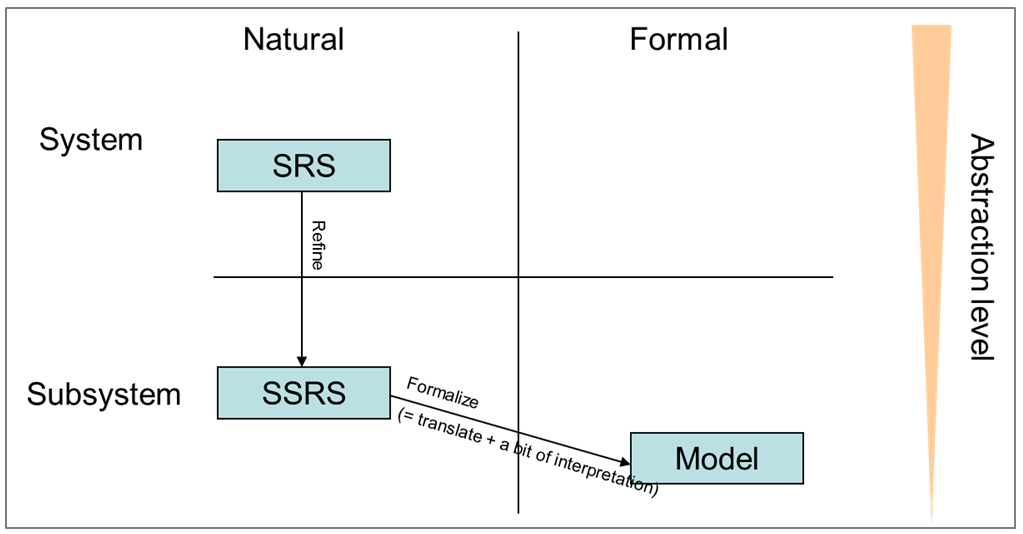
\includegraphics[width=15cm]{figs/abstraction_level}
The first outcome of this Task force will an overview of all necessary documents from the operator, the industry and all the European Railway Authorities to manage this kind of a documents.

\section{Objectives:}
The SSRS will be composed of two parts: 1/ the functional decomposition and the API (architecture) and 2/ the requirements.\newline
The functional decomposition \& API (architecture) is a functional breakdown of the subsystem. It makes explicit the boundaries of the onboard subsystem itself, and also provides the internal functional allocations (architecture) of this subsystem. This internal decomposition \& API (architecture) is composed of functions and flows of data between these functions. From the API we will derive the limits of this System.

All the objects described will be unambiguously named (in particular I/O) in a data dictionnary. 

This functional decomposition will be described using a semi-formal language.

This allocations (architecture) is useful for the following reasons:
 
\begin{itemize}
\item	it makes the system easier to maintain;
\item	it provides the boundaries of the system;
\item	it eases the safety analyses and the V\&V (with the internal cut out, and the unambiguous flows of data);
\item	it also helps  with modeling by providing some structure.
\end{itemize}
The second part of the SSRS is the requirements list. The requirements from the SRS are allocated toward the functions of the SSRS (the architecture), possibly split and rewritten in order to restrict their scope to these functions (of course, traceability is mandatory). They are also rewritten in order to match the objects named in the architecture (in particular internal and external I/O). The requirements are provided in natural language (even if the objects are unambiguously named). The formalization layer is coming below the SSRS, with the model.
 
The architecture objects (functions, streams...) and the requirements are tagged Vital/Non Vital.

\section{Organisation of the work}
The Task Force will be split in 4 Tasks:

\textbf{Task 1:} delivering of the Primary sources and the ERTMS knowledge from the industry and the operator. 
Operators and Industry – running parallel

Responsible: SSRS Task Baseliyos Jacob, Bernd Hekele, Deutsche Bahn???

List of Primary sources:
\begin{itemize}
\item ERA documents (subset 26 necessary requirements 4.5.2 + other documents)
\item Experience of the Operator 
\item Experience of the Industry
\item Operation Rules of the Operator
\item API /
\item Hazard Analysis from the Operator
\end{itemize}
\textbf{Task 2:} Functional Analysis: (2.5 PY)\\
Identification of the functions (to be realized in the kernel)\\ including inputs/outputs variables\\
Identification of the relationships between the functions\\
Creating of an consistent data dictionary\\
Clarify the requirements (describe the functions in a clear way)\\
Responsible: ERTMS Solution\\
Participants: All4Tec, CEA, ERSA, Lloyds/NS, DB, (SQS), (Systerel)\\
Reviewer: Alstom, DLR, Siemens, TUBS, (SNCF)

Output:\\
\hspace*{10mm}Data Dictionary (Database) (Attributes???)\\
\hspace*{10mm}Function (Database)\\
\hspace*{10mm}Link between Functions and Datas\\
\hspace*{10mm}Set of clarified requirements (Excel sheet)


Input: \\
\hspace*{10mm}Requirements on the tool:\\
\hspace*{10mm}Attributes??\\
\hspace*{10mm}Data check\\
\hspace*{10mm}Traceability\\
\hspace*{10mm}Multiuser\\
\hspace*{10mm}Reliability for integration\\
\hspace*{10mm}Flexibility of the database\\
\hspace*{10mm}Reporting\\
\hspace*{10mm}Change Management

\textbf{Task 3:} Documentation of the openETCS System Boundary:\\
Deriving all the interface specifications from the data dictionary\\
Defining the scope of the SSRS \\
Finalization of the SSRS\\
Responsible: DB\\
Participants: TUBS, DLR,\\ 
Review: Siemens, Lloyds/NS, All4Tec, Fraunhofer, TWT,

Input:\\
\hspace*{10mm}Data Dictionary

Outcome:\\
\hspace*{10mm}OpenETCS Interface specification\\
\hspace*{10mm}Functional architecture

Requirement on the tool:\\
\hspace*{10mm}Reliability for integration\\
\hspace*{10mm}Change Management
\newpage
\textbf{Task 4:} linked with WP 4 V\&V

\begin{tabular}{|  l || l | l | l | l | }
    \hline
    Task 1 &  &  & & \\ \hline
    Task 2 & ERTMS Solution & Lloyds&ERSA &DB \\ 
     & (ERTMS Experts) & (ERTMS Experts) & (ERTMS Experts) & (Operator
ERTMS Experts)
\\ \hline
    Task 3 &  &  & & \\ \hline
    \hline
  \end{tabular}
  \newline
  \\
    Pic  - Task overview
    \newline
  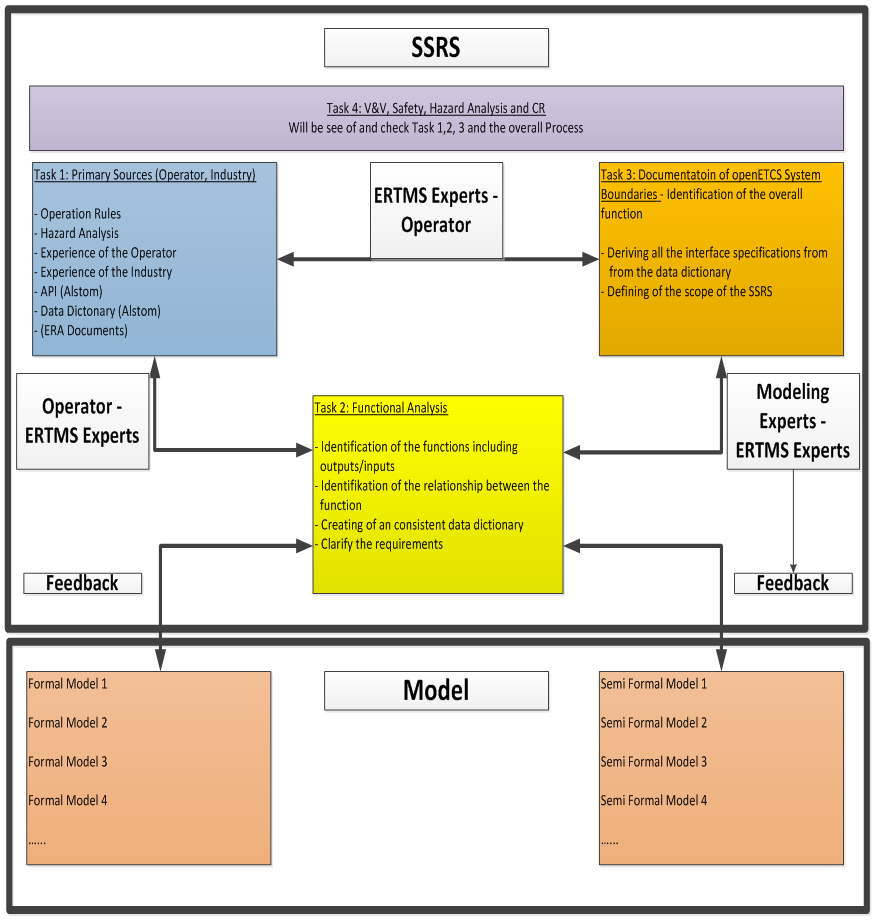
\includegraphics[width=15cm]{figs/task_overview}
  
  Note: the semi-formal and fully-formal modeling teams in tasks 3.5 and 3.6 should provide feedback to Tasks 1..4 during the whole project, and act as a reviewing team.

Actually, these teams are the customers of the SSRS team, as SSRS is the input for semi-formal model(s) and fully formal model(s).\\
\newpage
Pic 2 – Steps of Process\\
 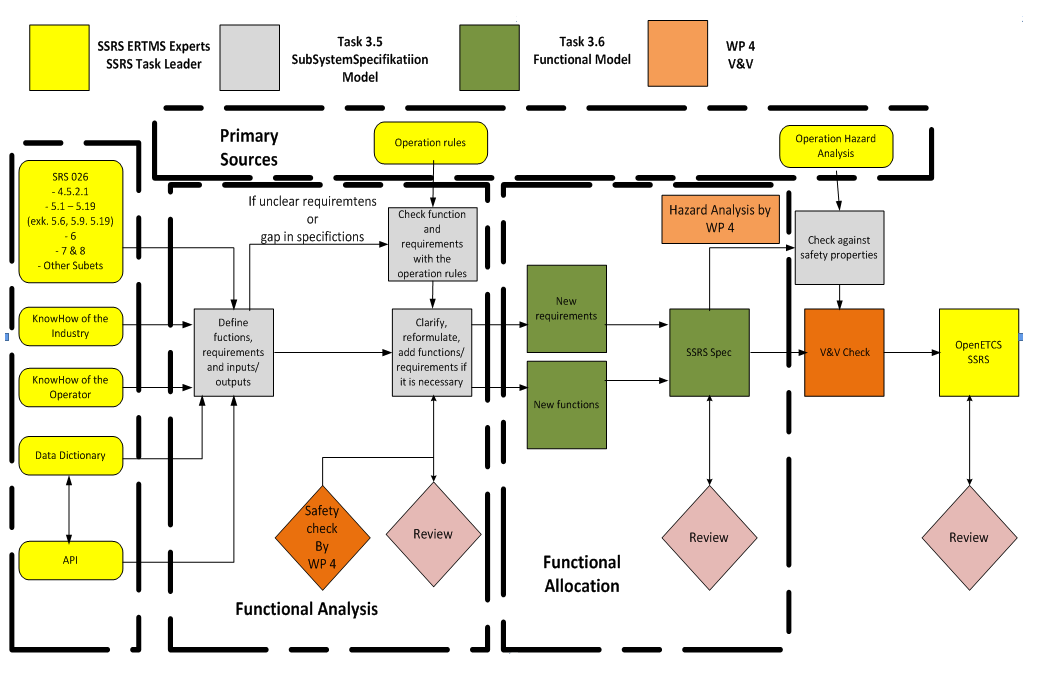
\includegraphics[width=15cm]{figs/Steps_of_Process}
 \\
 
 Pic  – Overall Process\\
 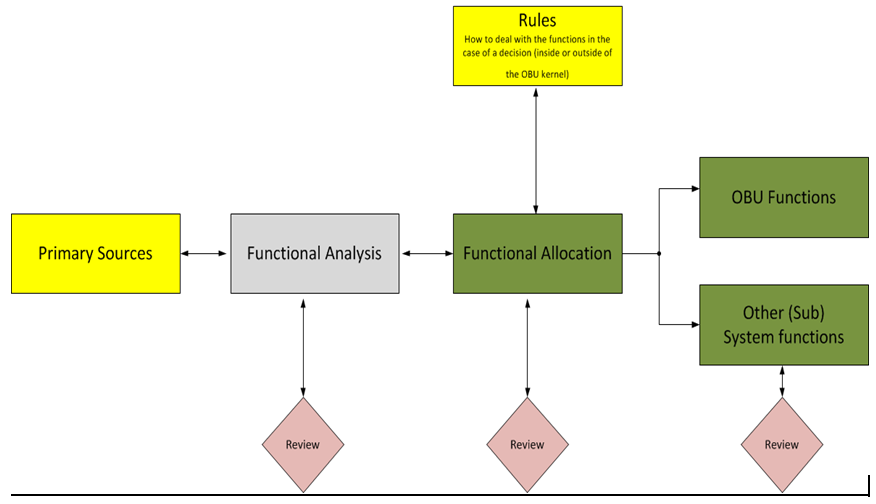
\includegraphics[width=15cm]{figs/Overall_Process}
 \newpage
 Pic  – Working Couples\\
 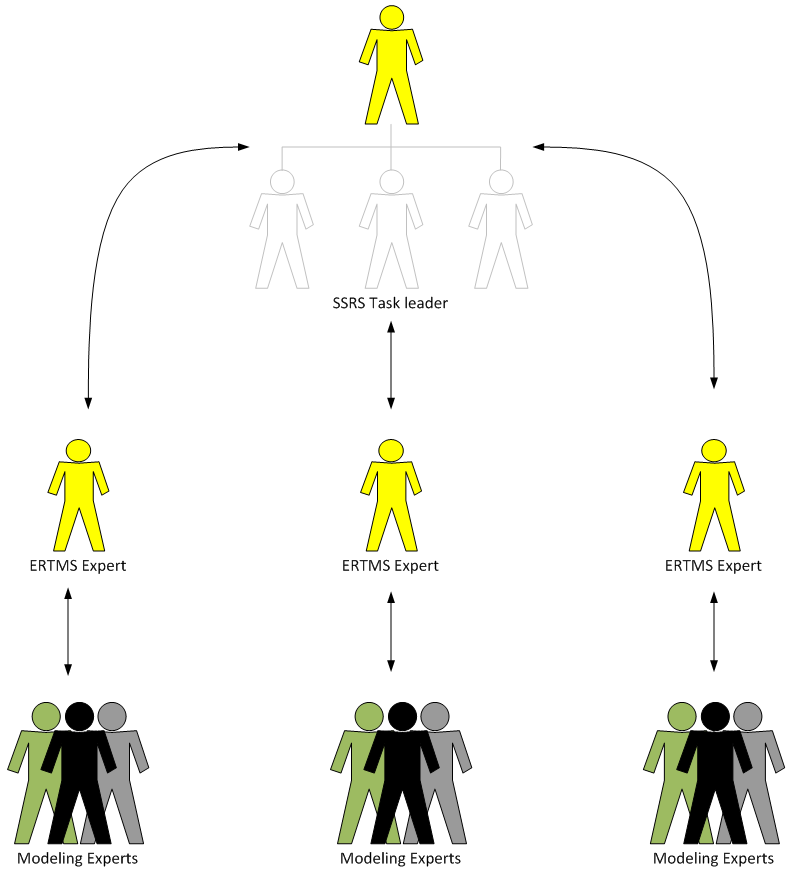
\includegraphics[width=15cm]{figs/Working_Couples}\\
 \subsection{Sprint List}
 \textbf{Main Requirements Sources\newline
 \begin{tabular}{|  l || l | }
    \hline
    4.5.2.1 Active FunctionsTable &   \\ \hline
    5.1 – 5.19 (exc. 5.6, 5.9, 5.19)Procedures &  \\ \hline
    6 Management of older systems &   \\ \hline
    7 ERTMS/ETCS Language &   \\ \hline
    8 Messages &   \\ \hline
    TSI Annex A &   \\ \hline
    \hline
  \end{tabular}}
 
  \newpage 
  \subsection{Goal}
  Weekly Telco (30 min.)\\
  Newsletter\\
  Short communication sessions between operator – modeler – ERTMS Experts


08/7- 19/7. Sprint 1

Sprint 1 shall include the following work:

Baseliyos Jacob and Stan. Pinte:
\begin{itemize}
	\item Put in operation a Temporary requirement tool
	\item Plan Next sprint tasks + schedule 
\end{itemize}
Task 1 team:
\begin{itemize}
	\item Gather operational and national rules documents
	\item Gather hazard analysis documents
\end{itemize}

Task 2 team:
\begin{itemize}
	\item Start graphical functional decomposition by modeling top-down the Subset-026, defining functions and data flows
\end{itemize}
Task 3 team:
\begin{itemize}
	\item Integrate + Reviewing ERA documents and Spread the Requirements from the SRS026 
	\item Integrate data dictionary from existing ERTMSFormalSpecs data dictionnary
\end{itemize}
\newpage
\subsection{Time Schedule}
Pic  – Working Couples\\
 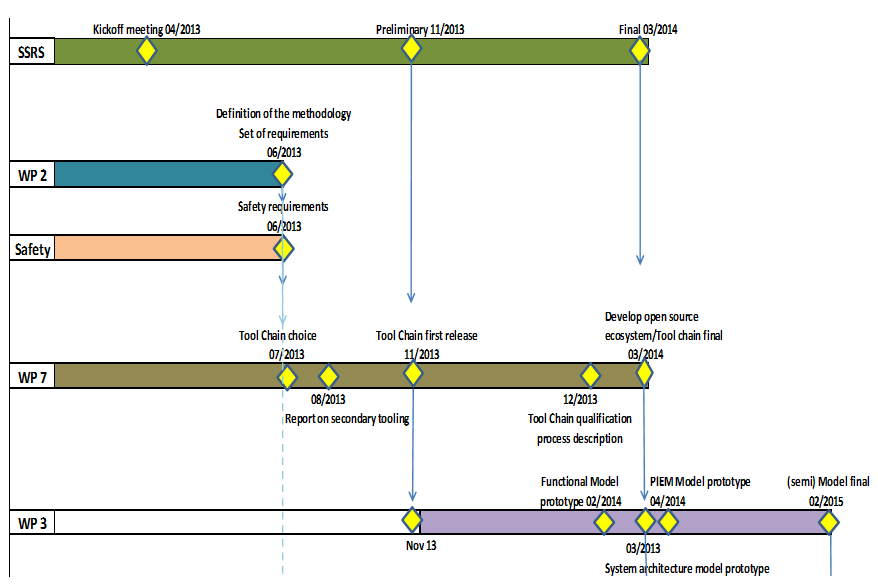
\includegraphics[width=15cm]{figs/time_schedule}
 
 \section{Requirement for SSRS Tools:}
 \subsection{Requirements for the SSRS Requirements Management tool.}
\begin{itemize}
  \item[-] Need an documents based outcome (Excel)
  \item[-] Must be compatible to a graphical decomposition and (semi) formal model tool
  \item[-] Version management
  \item[-] Multi user
  \item[-] Data Dictionary Check
\end{itemize}
\begin{itemize}
  \item[ ]\textbf{\underline{Attributes:}}
  \item[-]Requirement ID
  \item[-]Document Source
  \item[-]Related SRS §
  \item[-]National Operation Rules xx country
  \item[-]Variable Name – Input Variable/Output Variable
  \item[-]Descritption
  \item[-]ETCS language reference
  \item[-]Version (Document)
  \item[-]Source (source of required information)
  \item[-]Range (possible values)
  \item[-]Source assumed (if source is not clear)
  \item[-]Comment
  \item[-]Proposal
  \item[-]Remark
  \item[-]User – Unique/Multiple
  \item[-]Discussion of the requirement in Subset 25 – xx ID
  \item[-]Functions
  \item[-]Functional Block
  \item[-]Validated
  \item[-]Informaton of requirement (need to/shall be)
  \item[-]approval
\end{itemize}
\subsection{Requirements for the SSRS Graphical Functional Analysis tool}
\begin{itemize}
  \item[-]Must be compatible to the requirement management and (semi) formal tool
  \item[-]Graphical Human interface
  \item[-]Data Flow Check
  \item[-]Data Dictionary Check
\end{itemize}

\section{Requirement on the SSRS at all}
The following is not part of the MoM, but is provided for the sake of completeness. This is an excerpt of the D2.6 – D2.9 document (current draft version).

\begin{itemize}
\item[\textbf{R-WP2/D2.6-X-10}] The SRS (SUBSET-026 for the reference baseline) shall be refined into a SSRS.
\item[\textbf{R-WP2/D2.6-X-10.1}] The SSRS shall provide a functional architecture of the OBU.
\item[\textbf{R-WP2/D2.6-X-10.1.1}] The SSRS shall split the KERNEL into independent functions.
\item[\textbf{R-WP2/D2.6-X-10.1.2}] The description of the architecture shall be semi-formal.
\item[\textbf{R-WP2/D2.6-X-10.1.3}] This architecture shall provide the functions and the data streams between them.
\item[\textbf{R-WP2/D2.6-X-10.1.4}] The SSRS shall describe which part of this architecture will be modelled.
\item[\textbf{R-WP2/D2.6-X-10.1.5}] The SSRS shall provide the interfaces between the considered subsystem and its environment.
\item[\textbf{R-WP2/D2.6-X-10.1.6}] When the boundary of the formalized subsystem corresponds to a FIS or FFFIS, the SSRS shall try to comply to it even when it is not mandatory.
\item[\textbf{R-WP2/D2.6-X-10.2}] The SSRS shall allocates the requirements of the SRS to the functions and their I/O.
\item[\textbf{R-WP2/D2.6-X-10.3}] Full traceability between the SRS and SSRS shall be provided.
\item[\textbf{R-WP2/D2.6-X-10.3.1}] Interpretations, additions and omissions shall be tracked and justified.
\end{itemize}
\textbf{
\underline{Architecture vs. functional decomposition}}


\textbf{\underline{Definiton of architecture}}\\
\textbf{\underline{What do we need?}}


\textbf{\underline{What is safety means? Robustness?}}

%===================================================
%Do NOT change anything below this line

\end{document}
